\subsection{HTB03 - Remote}
\subsubsection{Escaneo}
En el proceso de escaneo de puertos se encontró 6 puertos abiertos, el puerto 21 con el servicio FTP, el puerto 80 con un sitio web, el puerto 111 y 135 del servicio RPCBind, el puerto 445 con el servicio samba y el puerto 2049 del servicio NFS.
\begin{figure}[H]
    \centering
    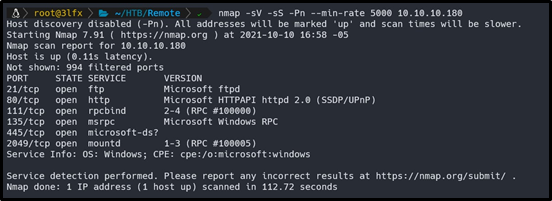
\includegraphics[width=0.99\textwidth]{imagenes/scanrem.png}
    \caption{Inyección de código malicioso en imagen}
\end{figure}
\subsubsection{Escaneo de puertos Remote}
Como primera acción se analizó el servicio FTP, donde se consiguió acceso anónimo, pero la ruta se encuentra vacía y no se cuenta con permisos de escritura.

Lo siguiente fue analizar el sitio web del puerto 80, allí se encontró referencias al CMS Umbraco, pero después nada más.
\begin{figure}[H]
    \centering
    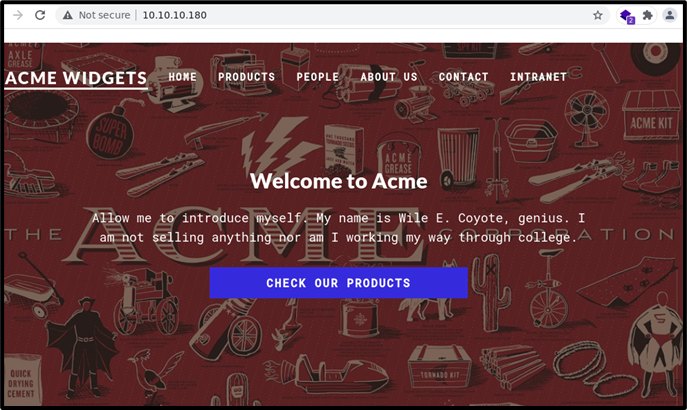
\includegraphics[width=0.9\textwidth]{imagenes/pagrem.png}
    \caption{Página web en Remote}
\end{figure}
Después se realizó enumeración de directorios con la herramienta Gobuster, obteniendo la ruta donde se encuentra el servicio Umbraco.
\begin{figure}[H]
    \centering
    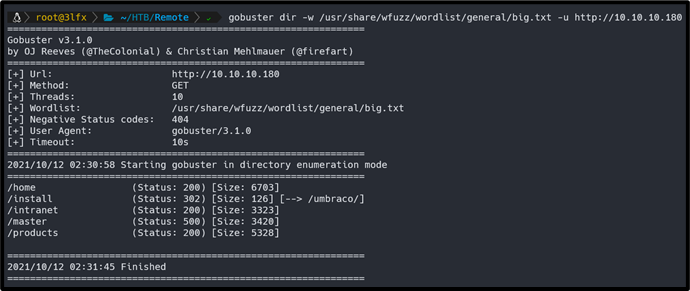
\includegraphics[width=0.99\textwidth]{imagenes/enudicrem.png}
    \caption{Enumeración de directorios en Remote}
\end{figure}
Con ello se procedió a dirigirse a la ruta encontrada, obteniendo un formulario para inicio de sesión.
\begin{figure}[H]
    \centering
    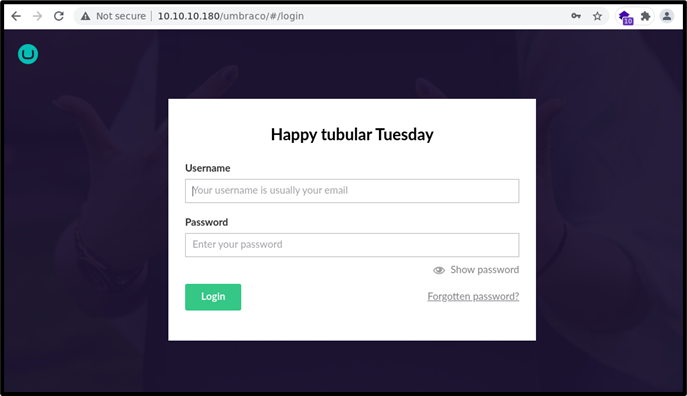
\includegraphics[width=0.99\textwidth]{imagenes/logumb.png}
    \caption{Página Login del servicio Umbraco}
\end{figure}
Se intentó usuario y contraseñas predeterminadas para acceder, pero no se tuvo éxito. Antes de intentar fuerza bruta se analizó el puerto 445 con el servicio samba, pero no se logró tener acceso.

\vspace{0.5cm}
Lo siguiente a realizar fue un escaneo RPCBind con el comando “rpcinfo”, donde se observó el servicio NFS del puerto 2049.
\begin{figure}[H]
    \centering
    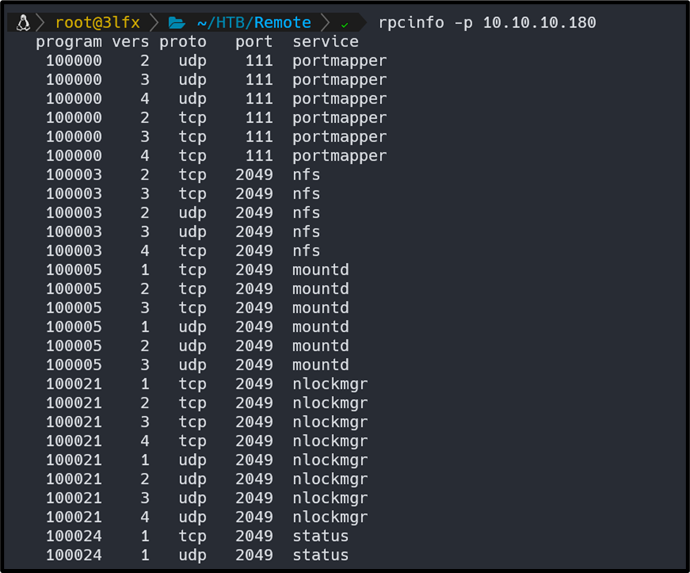
\includegraphics[width=0.99\textwidth]{imagenes/rpcrem.png}
    \caption{Escaneo RPCBind en Remote}
\end{figure}
A continuación, se comprueba si hay algún recurso compartido disponible para montar utilizando la herramienta “showmount”.
\begin{figure}[H]
    \centering
    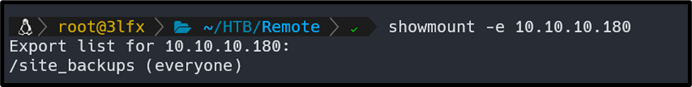
\includegraphics[width=0.99\textwidth]{imagenes/shmonrem.png}
    \caption{Directorio disponible de Remote para montar}
\end{figure}
Como se muestra en la imagen anterior, se encuentra el directorio “site\_backups” para montarlo en nuestra máquina atacante.
\begin{figure}[H]
    \centering
    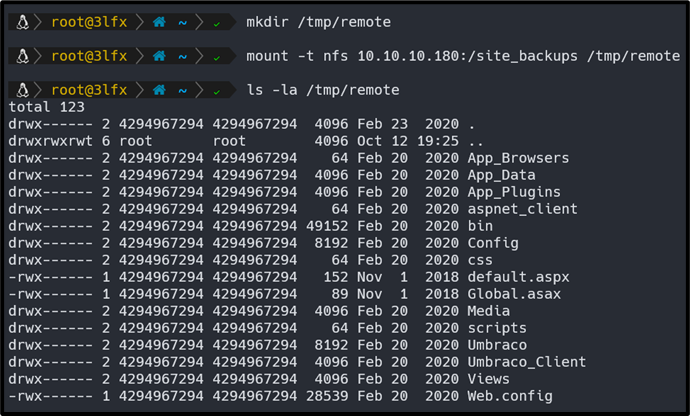
\includegraphics[width=0.99\textwidth]{imagenes/revdicrem.png}
    \caption{Revisión del directorio montado de Remote}
\end{figure}
Al revisar el directorio montado se puede observar que es un “backup” del sitio web. Buscando información en internet sobre donde se almacena la base de datos en el CMS Umbraco, se identificó que esto se ubica en un archivo con extensión “.sdf” en el directorio “App\_Data”. Cuando se lee el archivo, se presentan caracteres no imprimibles, por ello se usa el comando “strings” para obtener la información importante y el comando “head” para leer solo 10 primeras líneas obteniendo lo siguiente.
\begin{figure}[H]
    \centering
    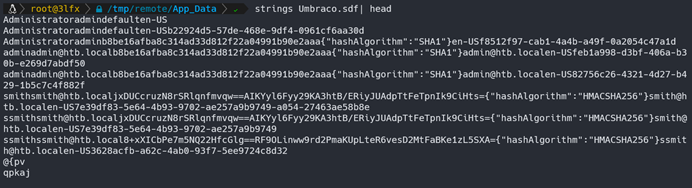
\includegraphics[width=0.99\textwidth]{imagenes/conumb.png}
    \caption{Contraseña en formato hash de Umbraco}
\end{figure}
Como se observa en la imagen anterior, se presenta la contraseña en formato hash del usuario “admin@htb.local”. Para intentar crackear la contraseña, se intentó mediante la página web “Crackstation” \cite{crack}, donde se obtuvo exitosamente la contraseña en texto plano (DE02).
\begin{figure}[H]
    \centering
    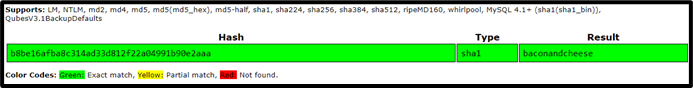
\includegraphics[width=0.99\textwidth]{imagenes/desumb.png}
    \caption{Contraseña descifrada de Umbraco}
\end{figure}
Una vez obtenida la contraseña que resulta ser “baconandcheese”, se procede a iniciar sesión a través del navegador para acceder al servicio Umbraco, teniendo éxito al lograr ingresar.
\begin{figure}[H]
    \centering
    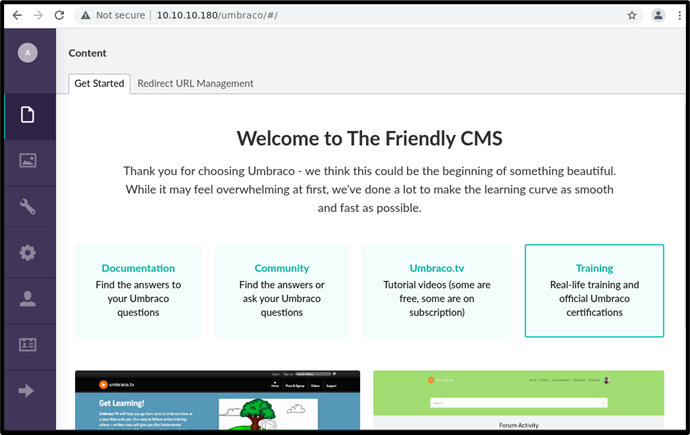
\includegraphics[width=0.99\textwidth]{imagenes/acumb.png}
    \caption{Acceso al servicio Umbraco}
\end{figure}
Cuando se obtuvo acceso, se revisó la página y se identificó que el CMS Umbraco utilizado era la versión “7.12.4”, con ello se procedió a buscar alguna vulnerabilidad en internet respecto a esta versión, encontrando que es vulnerable a ejecución remota de código (VU04).

Esta vulnerabilidad es debido a que esta versión de Umbraco permite realizar una inyección de XSLT a través del archivo “xsltVisualize.aspx” cuya ruta específica es “/umbraco/developer /Xslt/xsltVisualize.aspx” en el sitio web, por ello se puede realizar ejecución de código arbitrario.
\clearpage
\subsubsection{Explotación}
Para la explotar la vulnerabilidad encontrada, se usó un exploit escrito en Python perteneciente al usuario “noraj” de GitHub \cite{umbraco}. Para ganar acceso a la máquina se va a ejecutar una Reverse Shell a través de un script de Powershell obtenido del repositorio “Nishang” perteneciente al usuario “samratashok” de GitHub \cite{invokepower}.

Se procede a levantar un servidor HTTP mediante Python para que se pueda subir el script de Powershell a la máquina víctima,  y se pondrá en escucha un puerto para obtener la Shell requerida. El comando para ejecutar con el exploit será el de descarga de Powershell y se le agregará su ejecución.
\begin{figure}[H]
    \centering
    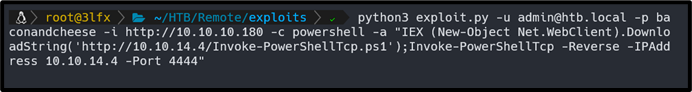
\includegraphics[width=0.99\textwidth]{imagenes/exprem.png}
    \caption{Ejecución de exploit Remote}
\end{figure}
Una vez que se descargó y ejecutó el script, se ganó acceso a la máquina como “iis apppool\textbackslash{}defaultapppool” como se puede observar en la siguiente imagen como prueba.
\begin{figure}[H]
    \centering
    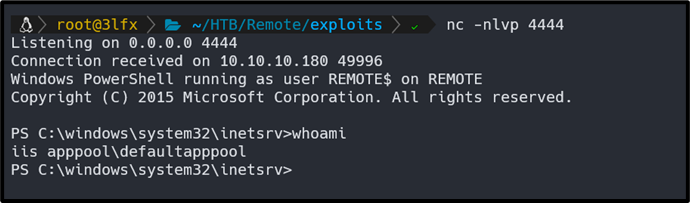
\includegraphics[width=0.77\textwidth]{imagenes/acrem.png}
    \caption{Acceso a la máquina Remote}
\end{figure}
\subsubsection{Escalamiento de Privilegios}
Para el escalamiento de privilegios, se utilizó el script “PowerUp.ps1” perteneciente a la organización “PowerShellMafia” de GitHub \cite{powerup} para identificar posibles configuraciones incorrectas que permitan el escalamiento de privilegios. Mediante el servidor levantado en la nuestra máquina atacante se descargó y ejecutó el script.
\begin{figure}[H]
    \centering
    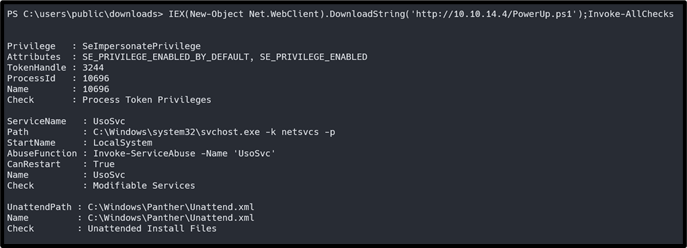
\includegraphics[width=0.82\textwidth]{imagenes/powerrem.png}
    \caption{Ejecución de sript ``PowerUp'' en máquina Remote}
\end{figure}
Del resultado de la imagen anterior primero se buscó como escalar privilegios mediante “SeImpersonatePrivilege”, donde se encontró el exploit “RogueWinRM” perteneciente al usuario “antonioCoco” de GitHub \cite{roguewin}, para ejecutarlo se le descargó mediante nuestro servidor y también se subió un ejecutable “nc64.exe” para generar una Reverse Shell, pero no se tuvo éxito en el intento.
\begin{figure}[H]
    \centering
    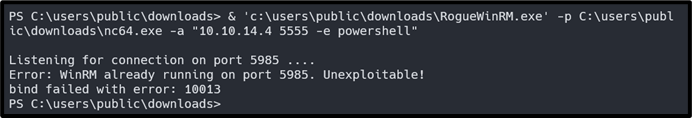
\includegraphics[width=0.99\textwidth]{imagenes/roguerem.png}
    \caption{Ejecución de ``RogueWinRM'' en la máquina Remote}
\end{figure}
El proceso siguiente fue investigar escalamiento de privilegios mediante “UsoSvc” donde se encontró que ese servicio al tener permisos incorrectos de archivo permite un escalamiento de privilegios mediante el reemplazamiento del binario (VU05).
\begin{figure}[H]
    \centering
    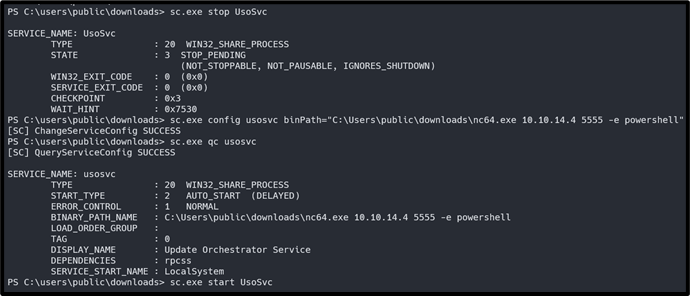
\includegraphics[width=0.99\textwidth]{imagenes/usorem.png}
    \caption{Modificación del servicio ``UsoSvc'' en Remote}
\end{figure}
Una vez modificado el binario para poder obtener una Reverse Shell con el “nc64.exe” que ya se contaba dentro, se volvió a iniciar el servicio y se consiguió obtener acceso al sistema como “nt authority\textbackslash{}system” teniendo como prueba la siguiente imagen.
\begin{figure}[H]
    \centering
    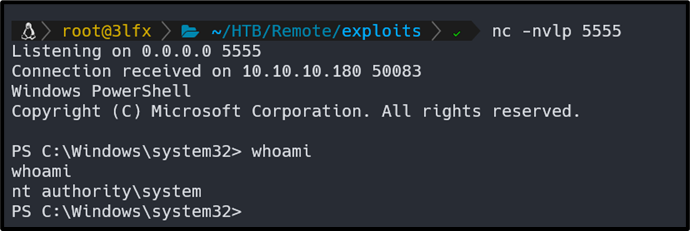
\includegraphics[width=0.8\textwidth]{imagenes/acntrem.png}
    \caption{Acceso como ``nt authority\textbackslash{}system'' en máquina Remote}
\end{figure}
Luego de aproximadamente 30 segundos, se detuvo el proceso de conexión mediante la Reverse Shell, y para evitar que suceda eso, se ejecutó de forma rápida otra conexión Reverse Shell en el tiempo que estaba activo la sesión con altos privilegios como se observó se tenía en la imagen anterior. Obteniendo de una conexión estable hacia la máquina objetivo.
\subsubsection{Post-explotación}
Como parte de la fase de post-explotación, se subió a la máquina victima un archivo ejecutable “mimikatz.exe” \cite{mimikatz} para conseguir extraer si es posible las contraseñas en texto plano o en su defecto los hashes NTLM de los usuarios de la máquina.

El resultado que se obtuvo fue que no se pudo conseguir contraseñas en texto plano debido a que marcaba error al intentar extraer información del proceso LSASS. Por ello se procedió a extraer los hashes NTLM de la base de datos SAM.
\begin{figure}[H]
    \centering
    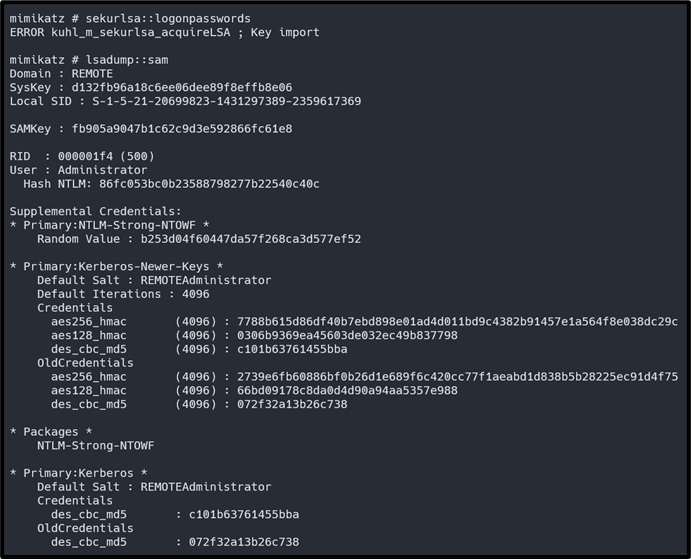
\includegraphics[width=0.8\textwidth]{imagenes/hasadrem.png}
    \caption{Contraseña en formato hash del usuario ``Administrador'' en Remote}
\end{figure}
De la extracción de información de SAM se obtuvo credenciales pertenecientes al usuario “Administrator” y del usuario “WDAGUtilityAccount”.
\begin{figure}[H]
    \centering
    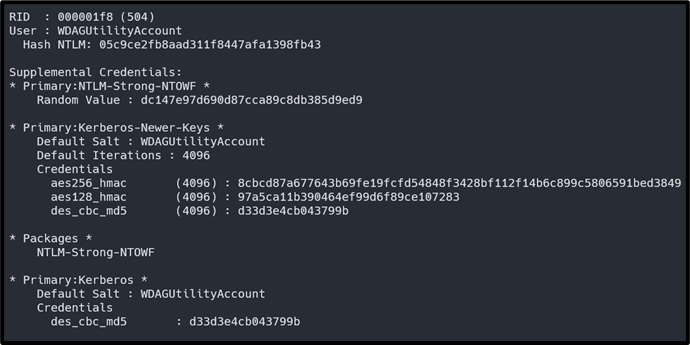
\includegraphics[width=0.8\textwidth]{imagenes/haswdarem.png}
    \caption{Contraseña en formato hash del usuario ``WDAGUtilityAccount'' en Remote}
\end{figure}
\subsubsection{Recomendaciones de mitigación}
Las recomendaciones para evitar ataques según las vulnerabilidades y debilidades encontradas son las siguientes:
\begin{itemize}
    \item No usar el servicio NFS para la exposición de backups porque no se cuenta con una verificación que controle quienes pueden acceder a los archivos, de preferencia que se use el servicio SMB para este propósito.
    \item Actualizar el CMS Umbraco a una versión más actualizada con la finalidad de evitar la ejecución remota de Código.
    \item Realizar un control en los permisos de los servicios para evitar la elevación de privilegios a un usuario.
\end{itemize}
